\documentclass{report}
\usepackage[utf8]{inputenc}
\usepackage{amsmath, amssymb}
\usepackage{graphicx}
\usepackage[margin=1.25in]{geometry}
\usepackage{multirow}
\usepackage{pdfpages}
\usepackage{float}
\usepackage{hyperref}
\hypersetup{
    colorlinks,
    citecolor=black,
    filecolor=black,
    linkcolor=black,
    urlcolor=black
}
\title{Lab \#6: Diffraction \& Interference Python Plotting}
\author{Neil Sawhney}
\date{December 2021}

\makeatletter
\def\@makechapterhead#1{%
  \vspace*{50\p@}% <----------------- Space from top of page to Chapter #
  {\parindent \z@ \raggedright \normalfont
    \ifnum \c@secnumdepth >\m@ne
        \huge\bfseries \thechapter.\ % <-- Chapter # (without "Chapter")
    \fi
    \interlinepenalty\@M
    #1\par\nobreak% <------------------ Chapter title
    \vskip 40\p@% <------------------ Space between chapter title and first paragraph
  }}
\makeatother
\begin{document}

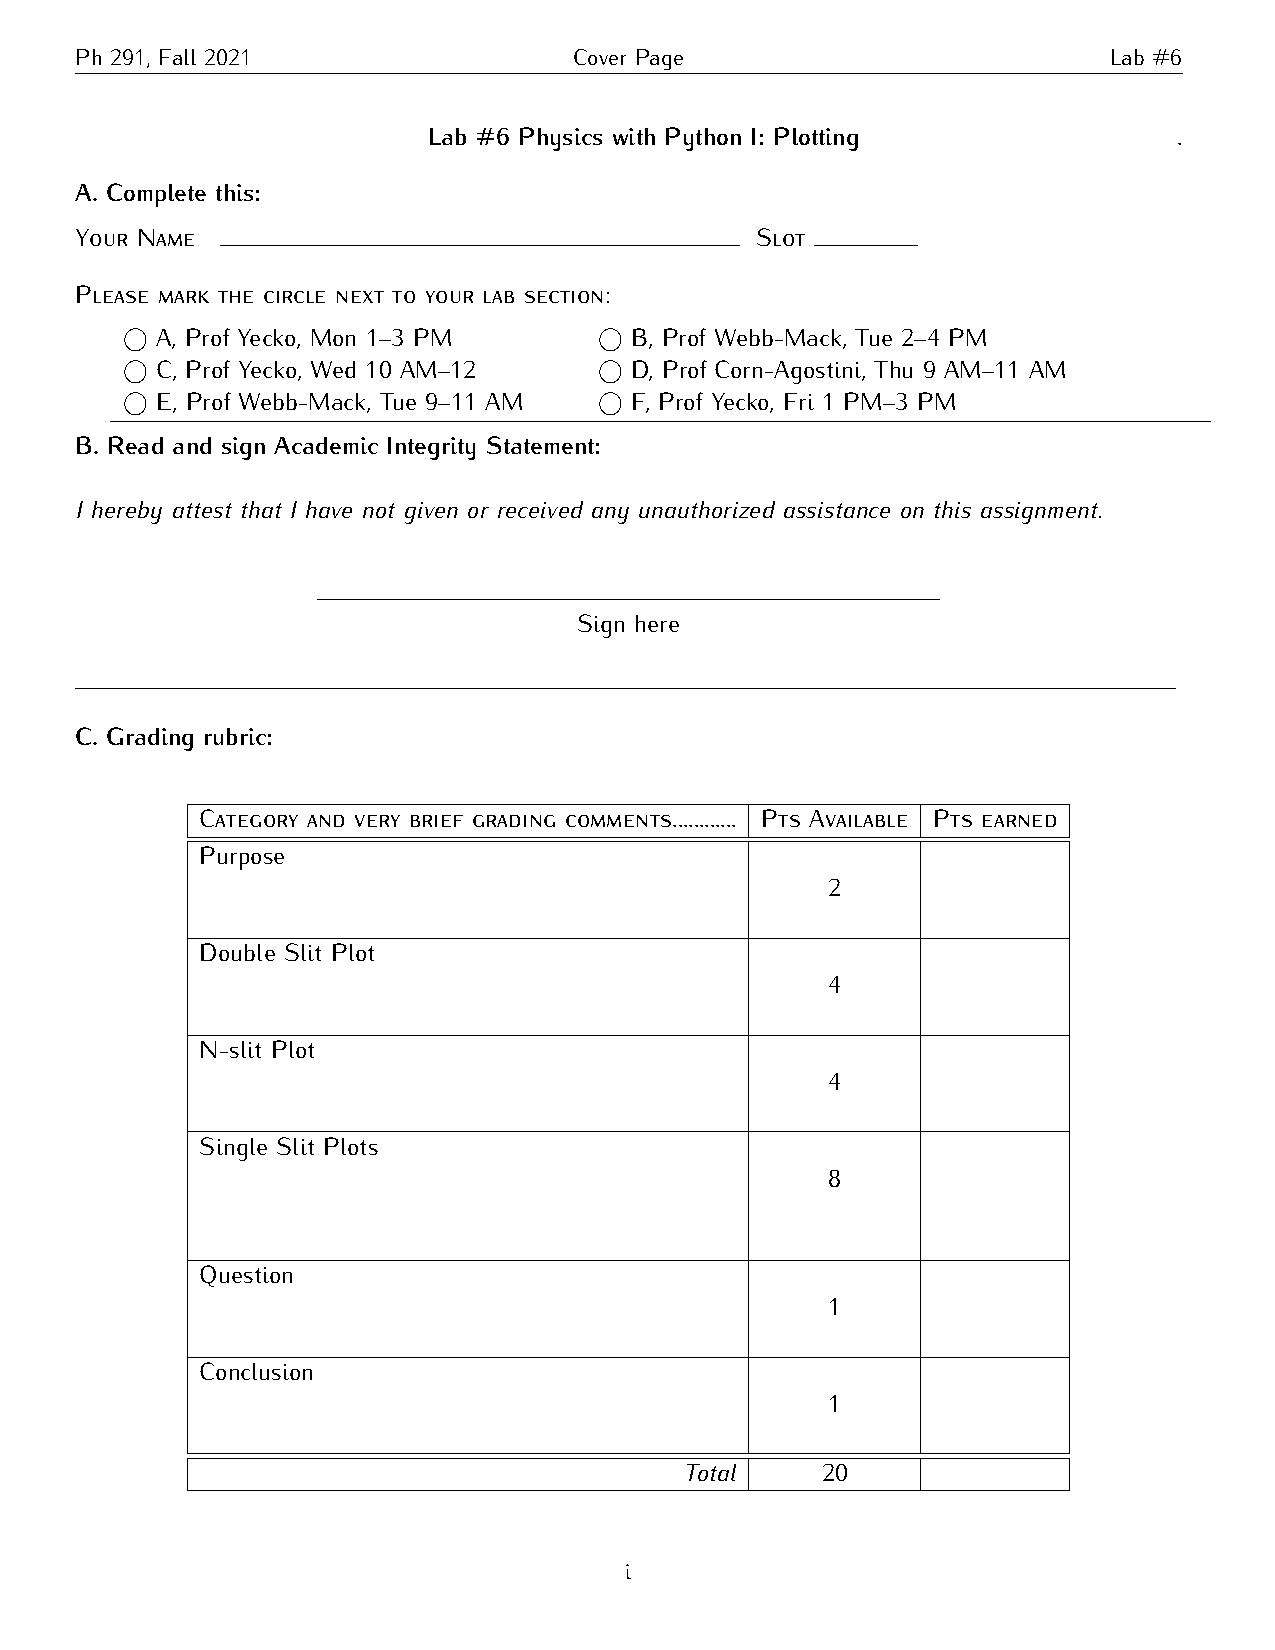
\includepdf[pages=-]{Lab6-COVER.pdf}

\maketitle
\tableofcontents

\chapter{Purpose}
The purpose of this lab is to plot the intensity pattern of light as it passes through 1, 2, and N number of slits for an infinitesimally small slit. Using these results we will plot the intensity pattern of light for a slit of finite width.


%-----------------------------------

\chapter{Results}

\begin{table}[H]
    \centering
    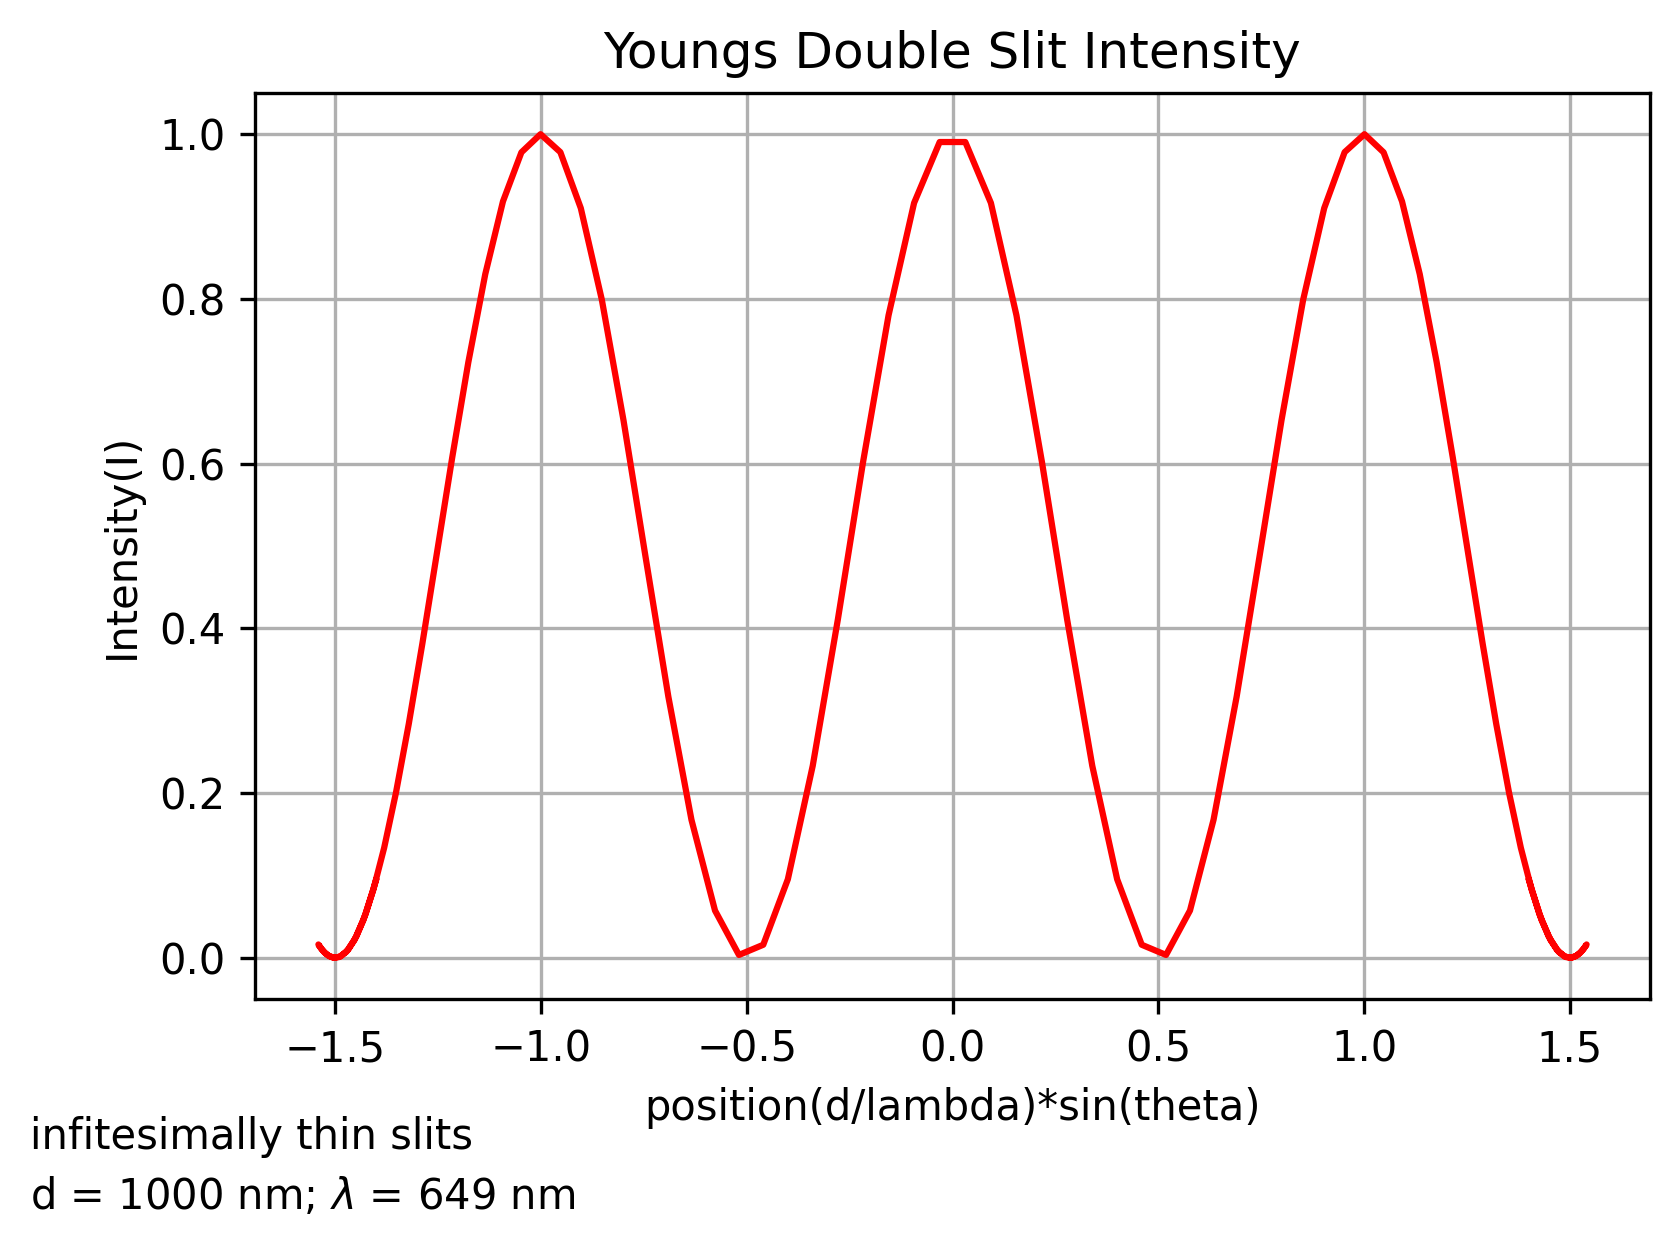
\includegraphics[width = \textwidth]{plot1.png}
\end{table}
\bigskip

\begin{table}[H]
    \centering
    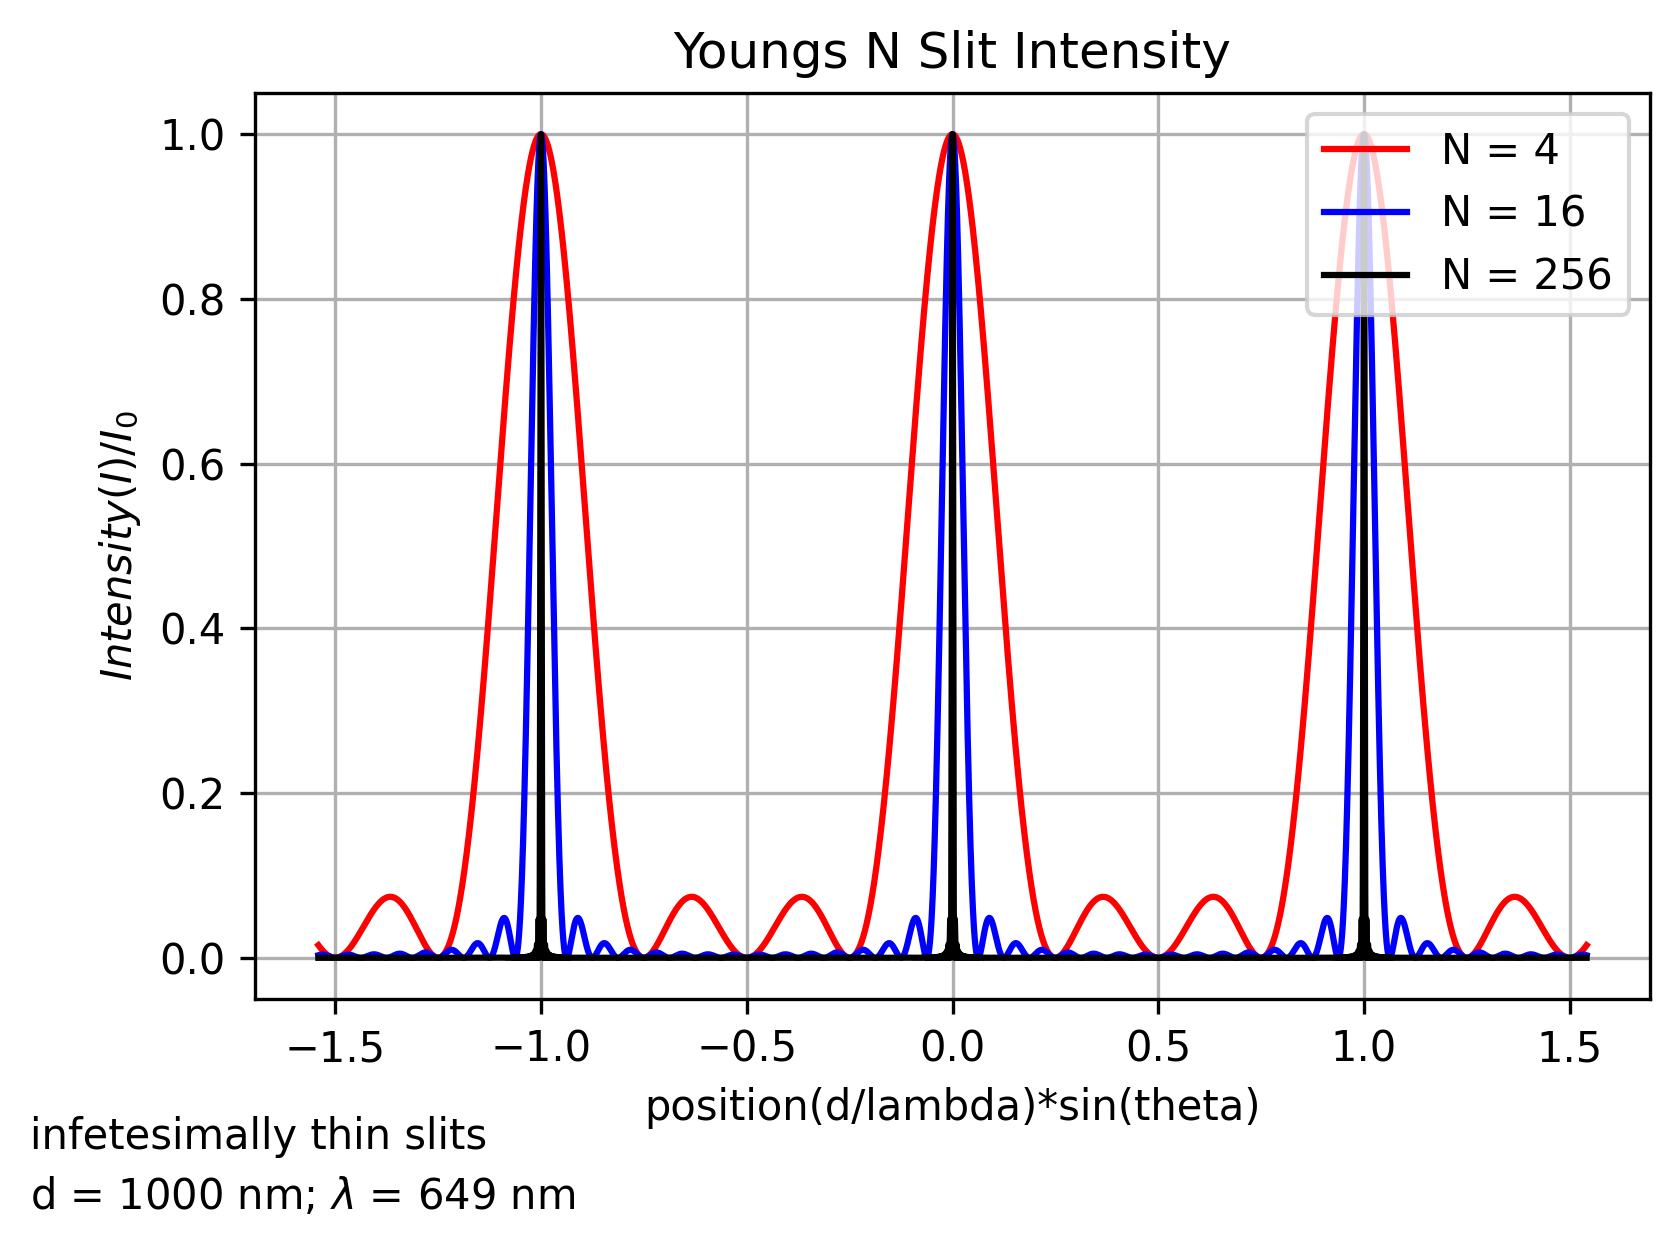
\includegraphics[width = \textwidth]{plot2.png}
\end{table}
\bigskip

\begin{table}[H]
    \centering
    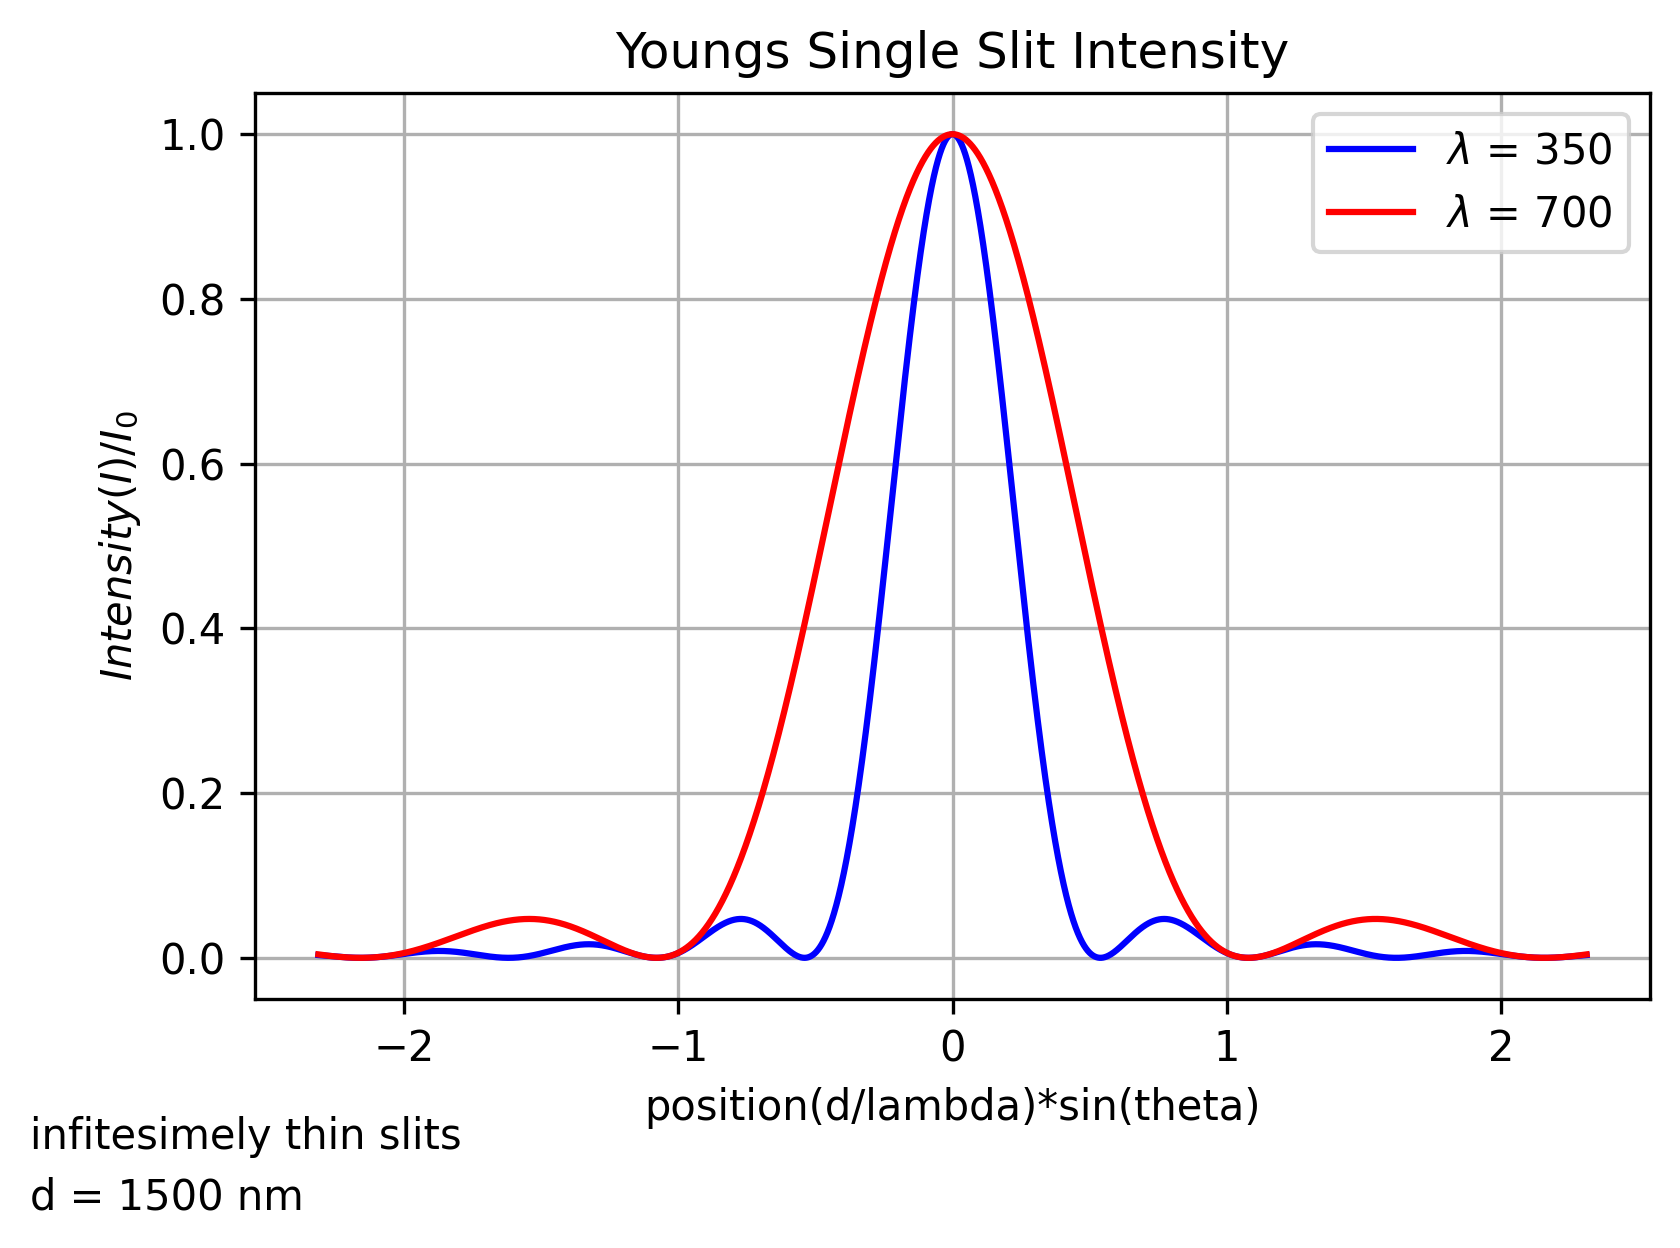
\includegraphics[width = \textwidth]{plot3.png}
\end{table}
\bigskip

\begin{table}[H]
    \centering
    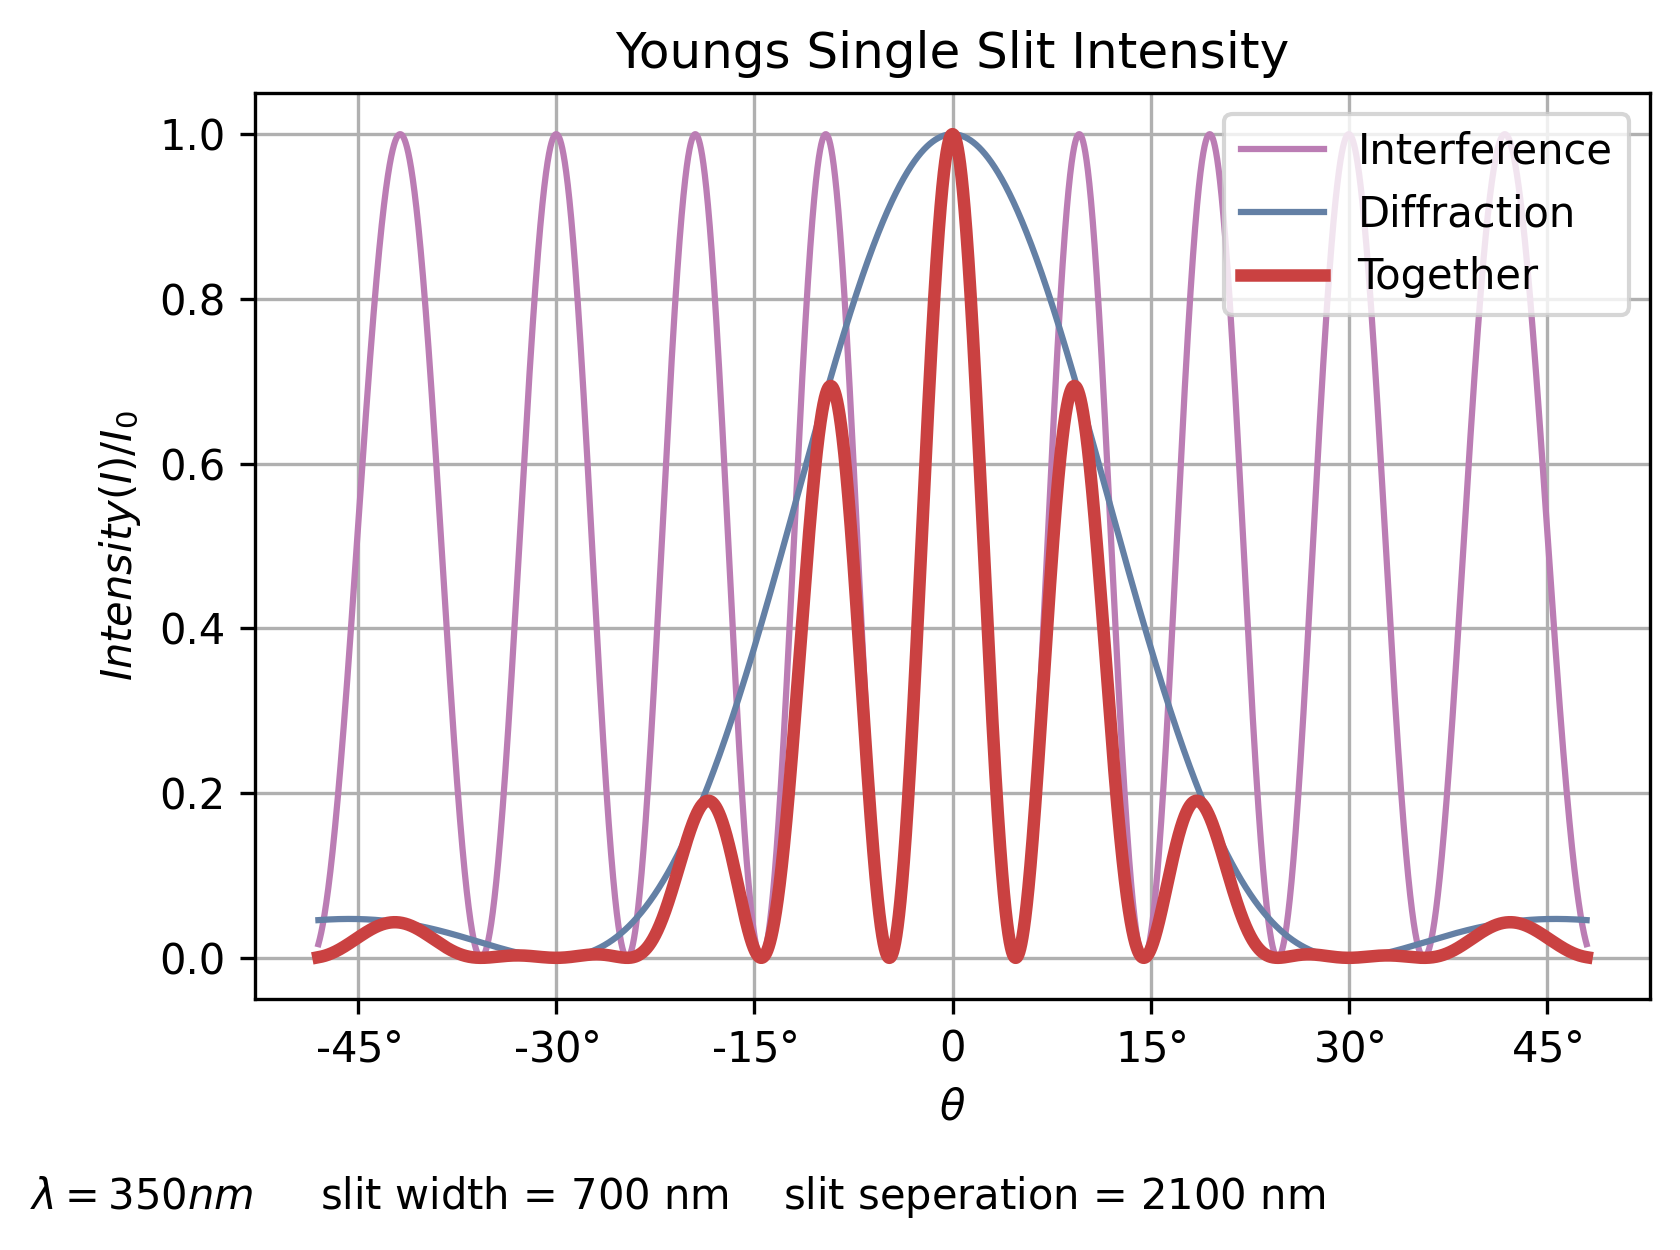
\includegraphics[width = \textwidth]{plot4.png}
\end{table}
\bigskip

\subsection*{Question}
\label{Question}
Notice that the m=3 ($\theta \approx 30^\circ $) order is missing. \\

\noindent The bright interference fringes occur at $d \sin \theta=m \lambda$, or

\begin{equation}
    \sin \theta=\frac{m \lambda}{d}
    \label{sin}
\end{equation}

    We also know that,
$$
I=I_{0}\left(\frac{\sin \beta}{\beta}\right)^{2}
$$
    where
\begin{equation}
    \beta=\frac{\pi a \sin \theta}{\lambda}
    \label{beta}
\end{equation}
    Substituting equation \ref{sin} into \ref{beta},
$$
\beta=\frac{\pi a \sin \theta}{\lambda}=\frac{\pi a}{\lambda} \cdot \frac{m \lambda}{d}=\frac{m \pi a}{d}
$$
For $a=2 \lambda, d=6 \lambda$, and $m=3$,
$$
    \beta=\frac{(3) \pi(2 \lambda)}{(6 \lambda)}=\pi
$$
Then, the intensity is
$$
    I=I_{0}\left(\frac{\sin \beta}{\beta}\right)^{2}=I_{0}\left(\frac{\sin (\pi)}{\pi}\right)^{2}=0
$$
Although the interference intensity in very high at this point, the diffraction inten:w
sity is 0 and cancels it out

\chapter{Conclusions}

A single slit of finite width can be plotted by multiplying the equation for a double slit of infinitesimally small width and a single slit of infinitesimally small width where d of the double slit is the slit separation and d of the single slit is the slit width.



\chapter{Answered Questions}
Click the question to be brought to the location where the question is answered.

\section{Question}
\hyperref[Question]{missing m = 3 order}

\end{document}
